\chapter{Einleitung}

Diese Dokumentation soll während des ganzen Projekt ergänzt und nachgeführt werden.
\section{Zweck dieser Applikation}
\begin{itemize}
\item Diese App ist für Verkündiger gedacht.
\item Es soll nicht als Ersatz der Dienstabmachungen mit der eigenen Versammlung dienen.
\item Diese App soll lediglich das finden eines Dienstpartners vereinfachen, wenn Verkündiger eine kurzfristige Dienstabsage erhalten oder wenn niemand für den Dienst zu einer bestimmten Zeit gefunden werden konnte.
\item Die App hat ihr Anwendungsgebiet innerhalb einer bestimmten Region, welche im Moment auf den Raum Zürich beschränkt ist.
\item Diese App soll auch Abmachungen mit einer Sprache, die nicht der Muttersprache entspricht, ermöglichen.
\item Der Grundgedanke die Dienstgruppe und die Einheit zu fördern soll bei der Implementierung der Applikation berücksichtigt werden.
\end{itemize}

\section{Projektaufbau}

Dieser Aufbau ist noch abhängig von gewissen Grundsatzentscheiden, ausserdem ist er eventuell noch nicht Vollständig \texttodo{Anna-Nina: Bitte ergänzen und überarbeiten. Visio File ist in Github repository doc/bilder}

\begin{center}
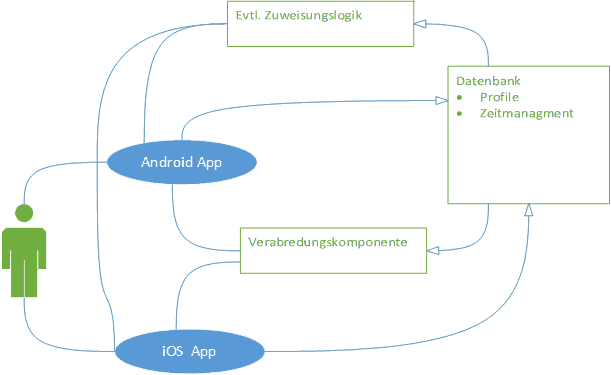
\includegraphics[width=0.5\textwidth]{bilder/useCase.png}
\end{center}
